\chapter{GPU Computing}

\section{OpenGL}
OpenGL is a cross-platform and open industry standard for programming two and
three dimensional graphics.\cite{OpenGL} The most common use of OpenGL is for programming on
dedicated graphics hardware. OpenGL is supported by all of the major graphics
cards makers, operating systems and game development studios.


Dedicated graphics hardware is generally a combination of special processors
and memory designed for the kind of vector processing commonly encountered in
graphics programming. One of the primary tasks in graphics programming is
rasterization. Rasterization is the process of representing a three-dimensional
scene as a set of discrete, two-dimensional pixels. While there are various
techniques for rasterization, an underlying theme is the necessity for a large
amount of independent calculations being done for each pixel. These operations
include many linear algebra and other floating point math operations useful for
two and three-dimensional geometry and effects.


As graphics hardware became more sophisticated, more control of this parallel
infrastructure has been given to the programmer. This became popular with the
advent of $shaders$, small programs which could be executed by the graphics
hardware to do more sophisticated computational operations than available
through the standard interface. Shaders were named for their primary use of
shading and lighting objects, which often times calls for the computation of
sophisticated mathematical and physical models. OpenGL provides a programming
language called GLSL for writing shaders, which allows the programer to
manipulate vertices, colors, textures, and recently geometry all in parallel.


\section{General Purpose GPU Programming}

use this citation (survey): \cite{Owens2007}

With the advances in graphics hardware, most notably with the introduction of
shaders, the GPU began to share similarities with the vector processing
architectures used in super computers for scientific simulations. Researchers
began using GPUs to compute problems suitable for a parallel vector processor
at a fraction of the cost of a super computer. The speed benefits of using a
GPU over a CPU for highly parallel problems at a low cost has generated
increasing interest in using the GPU for general purpose computing.
\toi{cite the cvt article evan talks about as well as a particle system on gpu article} 

\subsection{Architecture}
The idea behind the architecture of a Graphics Processing Unit is to have many
smaller floating point processors operate on a large amount of data in
parallel.
The way this is achieved in general is by implementing a memory heirarchy which
allows each processor to quickly operate on data which it needs. An abstraction for such a memory model is given in figure X:

\begin{figure}[!htc]
 		\centering
		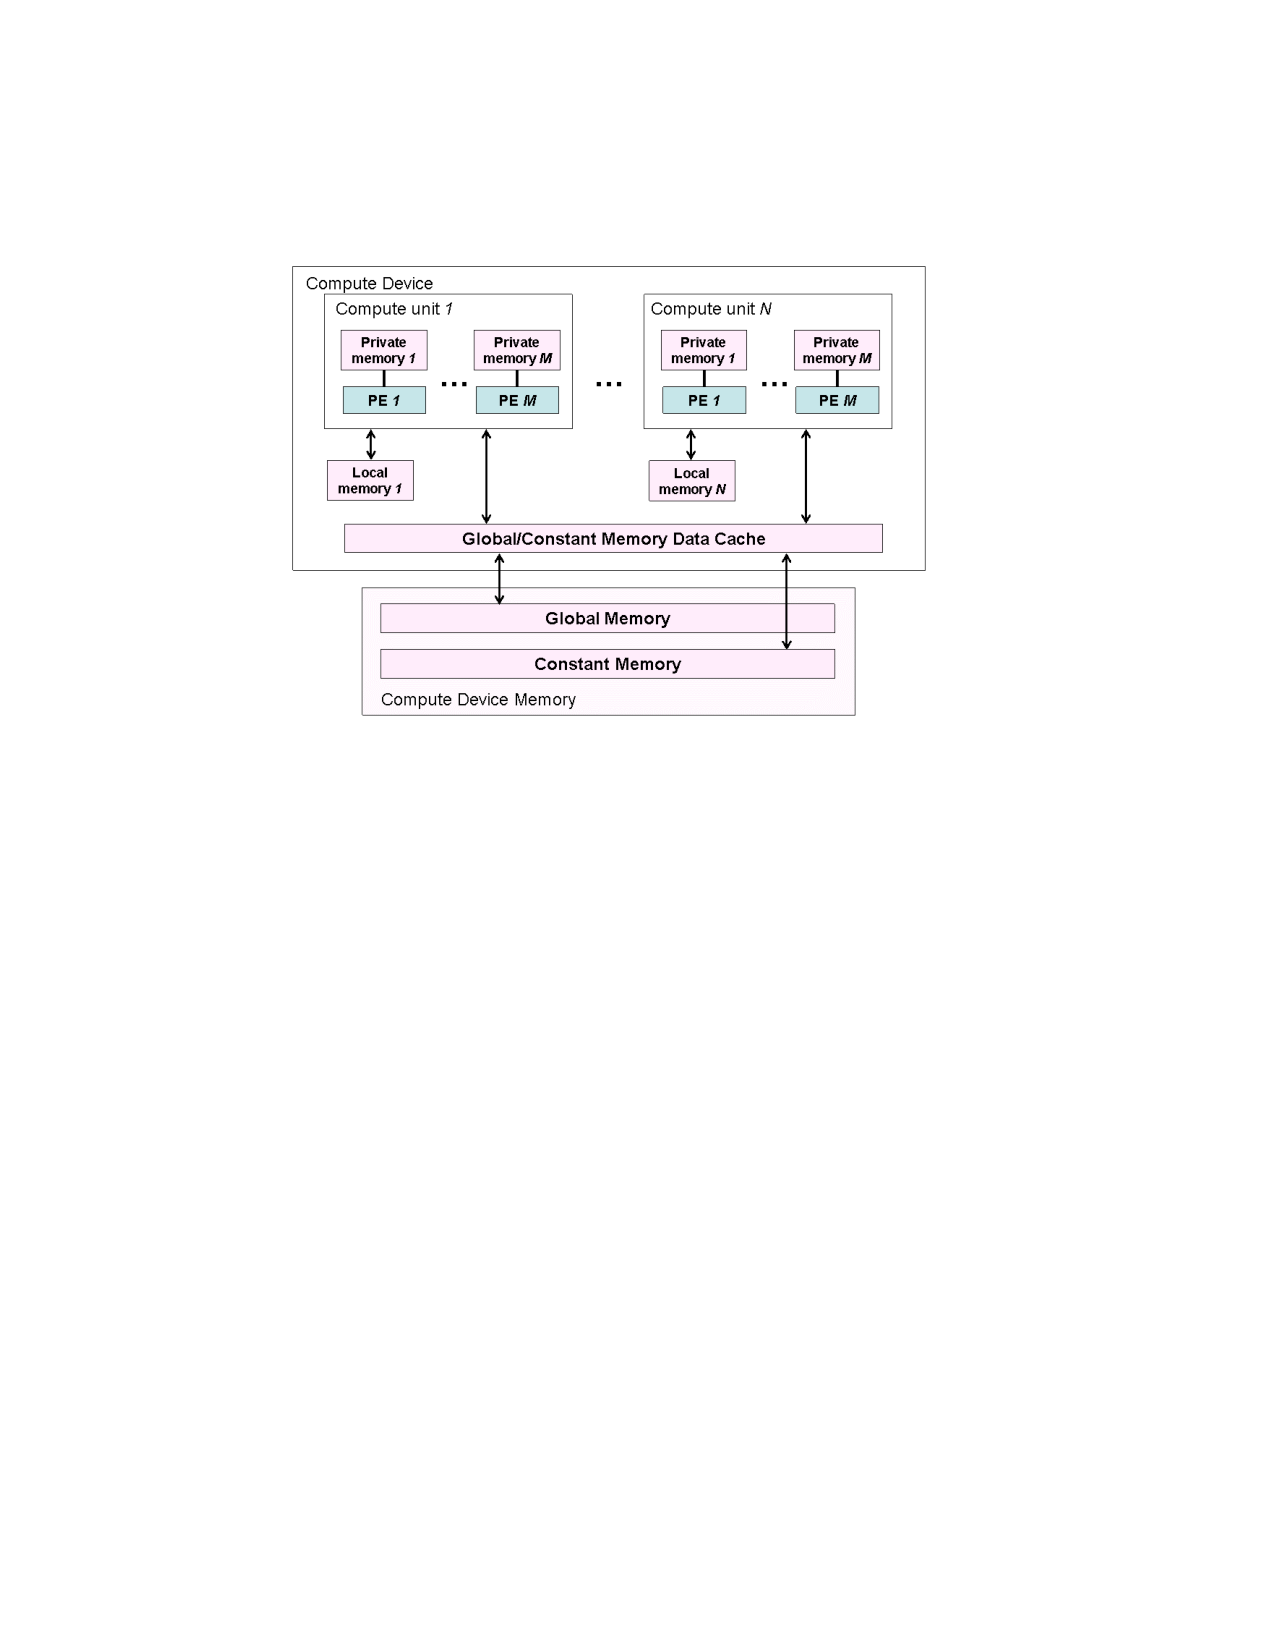
\includegraphics[scale=1.0]{figures/gpu_memory.pdf}
		\label{fig:logic}
        \caption{ OpenCL Memory Heirarchy Diagram \cite{OpenCLSpec} }
\end{figure}

The figure shows four main types of memory: $global$, $constant$, $local$ and
$private$. $Global$ memory is memory available to all of the processors (known
as compute units) and is the slowest type of memory in the heirarchy.
$Constant$ memory is memory which is read-only by the compute units, and is
usually cached for fast access. $Local$ memory is specific to each compute
unit, while much faster than $global$ memory it cannot be used to communicate
between compute units. Compute units are further divided into workers, which
can be thought of as individual threads which each have their own $private$
memory. Threads are executed in batches called workgroups, and each thread in a
workgroup has access to the same bank of $local$ memory, as well as access to
all of the $global$ memory. 


Since $local$ memory access is normally at least an
order of magnitude faster than $global$ memory access, GPU computing requires
great attention to the memory usage patterns of an algorithm. The most ideal
algorithms for general purpose GPU computing are Single Instruction, Multiple
Data (SIMD) algorithms in which the same operations are carried out on
completely independent data. For these algorithms each worker can operate on
the data assigned to it without concern for the behavior, status or output of
other workers. There exist many algorithms which are not completely SIMD but
can take advantage of the parallel nature of GPU programming by utilizing the
memory heirarchy in efficient ways.


\section{OpenCL}

OpenCL is a recent open standard for a parallel computing language and runtime
API put forward by the Khronos, an industry run consortium which also controls
the OpenGL standard.\cite{OpenCL} The OpenCL specification provides for two things, the
OpenCL runtime and the OpenCL programming language. The OpenCL runtime is
designed for parallel programming in heterogeneous environments, providing
mechanisms for dealing with multiple and varied compute devices such as CPUs
and the many types and generations of GPUs.  The OpenCL programming language is
a derivative of C99, giving it familiar syntax in an otherwise unfamiliar
context for many programmers.


In order to execute programs written in OpenCL a programmer must first use the
OpenCL runtime API to setup a $context$. An OpenCL context provides the
programmer with resources available from $devices$ within that context (such as
a GPU). The programmer may send memory as well as programs to the context
through the use of a $command queue$. Commands in the command queue may be
executed synchronously or asynchronously at the programmers behest. The most
important items manipulated in the command queue are $kernels$ and $buffers$.
Kernels are the OpenCL programs which will be executed on a particular device
while buffers are the memory which the kernels can take as arguments (i.e.
arrays). Kernels are compiled at runtime by OpenCL, allowing the same code to
be run on different device architectures without any guidance from the
programmer.


\subsection{CUDA}
Several years before the advent of OpenCL, graphics card manufacturer NVIDIA created the CUDA
language and runtime for general purpose computing on NVIDIA GPUs. CUDA is much
more specialized towards GPU computing than OpenCL, and also more mature as a
programming language. CUDA provides such programming language features as
Templates as well as an integrated programming environment for writing GPU code
inside of an otherwise CPU based program. The performance of CUDA on NVIDIA
cards is generally considered to be better than OpenCL, however it cannot be
run on other platforms such as those made by AMD or Intel. Due to CUDA's
proprietary nature and lack of availability on a sizeable section of the
computing population it was not considered as an option for this project.


\subsection{C++ Wrappers}
The OpenCL runtime libraries provided by the two largest GPU manufacturers are
written in C and can be utilized by including the standard C header files
provided by Khronos.\cite{OpenCL} Khronos also provides a set of C++ headers
which define convenient C++ classes for interacting with the OpenCL runtime. 


While the Khronos C++ headers simplify access to the OpenCL runtime API, for
many common uses further abstraction are convenient. In this project a set of utility classes are developed to simplify access to OpenCL resources. An example of such a simplifcation can be seen with the code for copying a standard vector to the GPU. With the Krhonos C++ API:
\begin{cppcode}{0}
     std::vector<float> a; 
     ... //initialize a 
     err = queue.enqueueWriteBuffer(cl_a, CL_TRUE, 0, array_size, &a[0], NULL, 
         &event);
\end{cppcode}
With the utility classes provided by this project:
\begin{cppcode}{0}
    std::vector<float> a; 
     ... //initialize a 
    cl_a.copyToDevice(a);
\end{cppcode}

These classes are described in more detail in the Implementation section of this thesis.


\subsection{CL/GL Interoperability}
A key performance consideration with GPU computing is memory transfer, as
discussed there is a large difference in speed between $local$ and $global$
memory, there is an even larger difference in the cost for transfering memory
between the host (CPU) memory and the device (GPU). Due to this cost it is
desirable to perform as many operations as possible on the GPU without needing
to transfer data between the host and the device.


As such a key feature in OpenCL programming for games is the ability to share a
context with OpenGL, allowing OpenCL to directly access and manipulate OpenGL
memory objects. With this feature one can avoid any transfer of data associated
with the graphics of the application, therefor if the computation done in
OpenCL changes the positions of objects to be rendered in OpenGL, it is all
done in the same memory location.


\subsection{Issues}
In the course of developing this project several small issues have been raised
whos solutions were not trivial. This section describes those issues and the
design decisions made to address them.

\subsubsection{Kernel Compilation Caching}
OpenCL is designed to compile kernels at runtime, and once those kernels are
compiled the binary version is cached for the context in which it is run. This
cuts down on the cost of running a kernel after the first compilation. An issue
arises with the Apple implementation of OpenCL when using include directives in
OpenCL code. If a kernel has been executed and cached by the Apple runtime,
changes to files included in the kernel will not be reflected in the following
run, indicating that the cache is not updated. Included files (such as header
files) are often used for isolating functionality which is common to many
routines, and it is desirable to develope this functionality in one place and
have all the code which uses it updated at once. With the caching issue this
style of development was not possible. The solution put forth in this project
was to use the g++ preprocessor to preprocess the OpenCL files after making
changes to the headers. This would generate OpenCL source files which had
everything in one file so that the kernel which OpenCL was caching was forced
to update. 


\subsubsection{float4}
The OpenCL 1.0 specification defines the \verb|float4| type as a vector of four
floating point numbers. Since the simulation in this project is designed to be
3 dimensional it is the most convenient data type for storing arrays of
coordinates. The OpenCL 1.1 standard does define a \verb|float3| type, but as
of this writing the 1.0 standard is still the most widely available
implementation so we use \verb|float4| for backwards compatibility. It is also
convenient to package many variables into a single array for use on the GPU,
and as such one may utilize the unused components of 3 dimensional vectors for
storing some scalar values.

\subsubsection{GL Context Sharing on the Mac}
The Apple implementation of OpenCL uses a specific extension for OpenGL context sharing which requires a specific way of creating an OpenCL context. The C++ headers provided by Khronos did not allow for this manner of Context creation, leading to the following modification of $cl.hpp$ provided by Khronos
\begin{cppcode}{1448}
Context(cl_context_properties* properties, cl_int* err = NULL)
    {    
        cl_int error;
        object_ = ::clCreateContext(
            properties, 0, 
            0,   
            NULL, NULL, &error);

        detail::errHandler(error, __CREATE_CONTEXT_FROM_TYPE_ERR);
        if (err != NULL) {
            *err = error;
        }    

    }    
\end{cppcode}

\subsection{Timing}

When developing a performance critical application it is important to know how
much time subroutines are taking to execute. OpenCL provides a mechanism for
timing the execution time of a kernel on the GPU, which is essential since
kernels may be executed asynchronously from the command queue. As part of the
convenience classes provided by this project for OpenCL, executing a kernel
automatically times its execution and returns the time in milliseconds.





